\chapter[Introdução]{Introdução}
% \addcontentsline{toc}{chapter}{Introdução}

Desde os primórdios da década de 50 e 60, a capacidade de armazenar, processar dados e informações de forma eletrônica evoluiu bastante. Se, por um lado, inicialmente o armazenamento e processamento de dados era restrito a um público técnico altamente especializado, atualmente existe uma série de ferramentas de apoio ao desenvolvimento de software voltados para o ambiente composto pela Internet, que servem aos mais variados propósitos, desde a simples divulgação de informações pessoais estáticas, perpassando as redes sociais com seus vários mecanismos de troca de informações, até chegar ao comércio eletrônico, no qual vários tipos de apoio a negócios são feitos nas mais  diversas áreas da atividade humana. 

Este capítulo procura motivar e justificar o estudo deste trabalho de conclusão de curso contemplando o contexto em que se inserem os CMSs.

\section{Motivação e justificativa}
\label{Contex}
Nesta seção são apresentadas definições básicas de plataformas de grande porte, sistema cliente-servidor e desenvolvimento web com o intuito de motivar e justificar a escolha do tema a ser apresentado na Seção \ref{Tema}.

%\begin{quotation}
%“Quanto ao significado de transporte coletivo urbano, embora não tenhamos encontrado uma definição legal específica para o termo, sua definição operacional abrange o transporte público não individual, realizado em áreas urbanas, com características de deslocamento diário dos cidadãos.” \cite{brasil2006}.
%\end{quotation}

\subsection{Plataformas de Grande Porte}
\label{Contex}
Um exemplo conhecido de desenvolvimento em grande porte é o uso de Mainframes, conhecidos por sua confiabilidade, estabilidade, segurança, disponibilidade e grande capacidade de processamento de dados. Os componentes de hardware de um mainframe têm capacidade de autocontrole e auto recuperação vastas. A confiabilidade do software do sistema é resultado de imensos testes e da capacidade de fazer atualizações rápidas para os problemas detectados \cite{shu_2013}.
	
Além do uso de mainframes, é importante destacar também os sistemas monolíticos, que, para \citeonline [p.~58]{Tanenbaum}, é uma “grande bagunça”, pois consiste apenas em um conjunto de rotinas, no qual cada rotina pode chamar qualquer uma das outras conforme a necessidade. Apesar da enorme capacidade de processamento, sistemas monolíticos são bastantes sensíveis a erros, pois, devido ao fato das rotinas poderem interagir com outras rotinas de forma muito fácil, quando há um erro, este erro se alastra rapidamente por todo sistema e assim pode causar a interrupção desse sistema.
	
Uma vantagem dos sistemas monolíticos é que a atualização ocorre de forma simples, pois basta atualizar a máquina  central e, como os terminais são sem capacidade de processamento local, toda a rede estará atualizada \cite [p.~58]{Tanenbaum}.

\subsection{Desenvolvimento Cliente Servidor}
\label{Contex}
De acordo com \citeonline[p.~58]{Tanenbaum}, os sistemas monolíticos eram desprovidos de grandes formalismos em suas estruturas, podendo pedaços de código (funções) chamar outros pedaços (funções) sem grandes restrições.

Com uma das motivações de reduzir a enorme quantidade de funções executadas pelo sistema operacional, foi proposto o sistema cliente servidor que, para \citeonline[p.~64]{Tanenbaum}, implementa a maior parte dos procedimentos do sistema operacional na forma de processos de usuário. \citeonline[p.~64]{Tanenbaum}, ainda acrescentam que no momento de solicitar um serviço, como executar uma determinada instrução de leitura, o processo de usuário (agora chamado de processo cliente) envia uma requisição para um processo servidor que então executa a tarefa e fornece uma resposta.

Para \citeonline{Duchessi_98}, o sistema Cliente - Servidor apresenta inúmeros benefícios. Alguns desses benefícios são:

\begin{itemize}
 \item Melhoria da acessibilidade do sistema.
 \item Redução de custos.
 \item Aumento da produtividade organizacional.
 \item Aumento na confiabilidade do Sistema.
\end{itemize}


Apesar de evitar a interrupção do sistema diante de um erro em alguma rotina, o sistema cliente - servidor apresenta alguns problemas. Um desses problemas é o fato de que, como existe processamento por parte do cliente, cada vez que se atualiza um sistema, todos os clientes devem ser atualizados, mesmo que isso seja feito de forma automática, o que foi uma das motivações para o surgimento dos sistemas web.

\subsection{Desenvolvimento Web}
\label{Contex}

De acordo com \citeonline{junior_2003}, a tecnologia Web funciona de forma relativamente simples, pois a Web é um conjunto de arquivos digitais que ficam armazenados em servidores ligados a Internet e que podem ser recuperados a partir de qualquer computador que tenha conexão com a Internet. Estes arquivos digitais são as chamadas páginas web que compõem a grande rede de informações que é a World Wide Web.

Os mesmos autores ainda afirmam que, com o passar do tempo, a Web foi adquirindo novos recursos e novas funções e houve um grande progresso quando os seus usuários passaram a não só solicitar páginas com conteúdo estático, mas também retornar resultados com conteúdo dinâmico.

\citeonline{Meusel_2008} dizem que uma dimensão importante para páginas web é manter um modelo consistente ao longo de todas as páginas. Aplicações web comuns consistem em elementos como um cabeçalho, um menu e um conteúdo da página agrupados em um esqueleto de página. Possuir uma separação estrutural em pedaços de HTML comuns e de código permite que tais pedaços possam ser compartilhados entre todas as páginas, o que traz um reuso para uma aplicação web de forma significativa.

Os sistemas web apresentam várias vantagens em relação aos demais sistemas \apudonline{Conallen}{perizo_2005}, diz que uma dessas vantagens é a manutenção, desenvolvimento e atualização centrada na aplicação. Isto é, diferente do sistema cliente servidor em que todos os clientes têm que ser atualizados quando o servidor é atualizado, nos sistemas web basta o servidor ser atualizado para que os clientes obtenham acesso as atualizações, reduzindo, assim, o custo de implementação das operações. Entretanto os sistemas web apresentam desvantagens. Uma desvantagem é que não há padronização para os navegadores de internet, o que pode acarretar em problemas de incompatibilidade dependendo de qual navegador está sendo usado e de qual versão é tal navegador\apud[p.~144]{Conallen}{perizo_2005}.


\section{Tema}
\label{Tema}
\citeonline{coelho2011} afirmam que qualquer conteúdo para ser divulgado e compartilhado na web, requer atenção especial das linguagens de programação a serem utilizadas. Na maioria das vezes o nível de complexidade para a construção de páginas web é alto e inacessível para leigos. Com esta motivação, em 1990 surgiram os sistemas de gestão de conteúdo (\textit{Content Management System}- CMS) que, para \citeonline{Barcia}, são plataformas que fazem a união entre diversos mecanismos os quais permitem criar e publicar conteúdo em tempo real em que, os usuários não precisam dominar uma programação específica para a construção de páginas na web, e além disso, possuem contato com páginas intuitivas e dinâmicas.

\citeonline{barrere}, declaram que sistemas CMSs oferecem diversos outros recursos. Alguns exemplos desses recursos são a fácil publicação e navegação por meio do conteúdo divulgado e a classificação de conteúdos em categorias. Além disso, pode facilmente agregar funcionalidades como blogs, ou fóruns de discussão.

Por oferecerem uma grande variedade de recursos, os CMSs são uma boa opção para quem deseja construir uma página web, pois permite que o desenvolvedor já inicie o projeto da sua página a partir de um determinado template. \citeonline{Nath_Arora}  ilustram que o processo de escolha de um CMS pode não ser algo simples, pois, além de existirem vários CMSs no mercado, cada CMS possui características únicas que podem ser decisivas para a montagem de uma aplicação específica, isto é, a escolha de um CMS pode influenciar em aspectos funcionais, de segurança, de desempenho, entre outros. Por esse motivo a criação de um método que auxilie o desenvolvedor a escolher um CMS faz-se necessário.  

%\textcolor{red}{\textit{Professor nesse parágrafo eu apenas conclui é necessário incluir alguma referência nele. }} 

%A partir disso o tema deste trabalho é estudar sistemas CMSs no contexto de desenvolvimento web visando a análise de desempenho desses CMSs.

\chapter[Definições]{Definições de Estudo}

Neste capítulo são definidos o problema a ser trabalhado, os objetivos gerais e específicos, a classificação da pesquisa, e o planejamento de como o trabalho será executado.

\section{Problema Abordado Dentro do Tema}
\label{probl}

%\textcolor{red}{Escrever aqui sobre as várias formas que existem para se criar uma página web. E destacar o uso de CMS como uma dessas formas. }
%
Para \citeonline{DePadua_2003}, o valor de um produto vem de suas características que, se tratando de software, podem ser funcionais ou não funcionais. Características funcionais representam os comportamentos que o sistema deve apresentar diante das ações de seus usuários. Características não funcionais definem determinados aspectos do comportamento que um sistema deve ter ao executar suas características funcionais. \citeonline{DePadua_2003} acrescenta que os requisitos funcionais explicam as funcionalidades que o produto deverá realizar em benefício daqueles que usam o sistema, enquanto que a especificação dos requisitos não funcionais completa os requisitos funcionais, descrevendo as restrições e outras características que o sistema deve possuir para que seja atingida a qualidade desejada.

%Dentre as várias classificações para requisitos não funcionais propostas por autores conhecidos na literatura, \citeonline{DePadua_2003} destaca um tipo relevante de requisito não funcional como sendo os requisitos de desempenho. Ele diz que, os requisitos de desempenho são requisitos numéricos, estáticos e dinâmicos, a que o produto ou o sistema maior devam obedecer e ainda acrescenta que todos os requisitos de desempenho devem ser especificados de forma quantitativa e mensurável.
%
Uma forma de enunciar objetivamente grandezas é a partir de medições. Neste sentido, a norma ISO 25000 expressa características em uso do produto, ou do próprio produto por meio de medições \cite{iso_25000}. 
%No contexto de desenvolvimento de software no Brasil o uso da \cite{Nbr_9126} apesar de pouco expressivo é o maior dentre todas as normas utilizadas por empresas de software que desejam alcançar a qualidade de seus produtos \cite{Marinho}. Os autores afirmam que 5,7 \% de 343 organizações pesquisadas utilizam a \citeonline{Nbr_9126} como padrão para se alcançar a qualidade de software.
%
%Assim sistemas web quando são construídos, também possuem características funcionais e não funcionais que descrevem um conjunto de requisitos que são definidos por um usuário.

Uma forma de construir sistemas web é com o uso de Sistemas Gerenciadores de Conteúdo ou \textit{Content Management System} (CMS), que permitem ao usuário construir sites para a internet com auxílio de vários modelos pré-concebidos de páginas web e diversos componentes pré-construídos. Seu uso concede ao usuário que deseja desenvolver páginas para internet flexibilidade, pois é possível que esse usuário separe o conteúdo da página do seu design, dentre outras vantagens. Como alguns exemplos disponíveis na indústria de software podem ser citados: Wordpress, Drupal e Joomla \cite{costa}.

A partir da motivação e tema propostos a questão de pesquisa é apresentada na Seção \ref{Declaração do Problema}, que vem logo a seguir.


\subsection{Questão de Pesquisa}
\label{Declaração do Problema}

A questão de pesquisa abordada por este trabalho é:

\textbf{{Como estabelecer um método objetivo para a escolha de CMSs a serem utilizados no desenvolvimento de sites Web?}}

\section{Objetivos}
\label{objEspp1}
Esta seção apresenta os objetivos geral e específicos do trabalho a ser desenvolvido.

\subsection{Objetivo Geral}
\label{Objetivo Geral}
Propor um método objetivo que possa servir de apoio para a escolha de um CMS. 

\subsection{Objetivos Específicos}

\label{objEspp2}
Para o Trabalho de Conclusão de Curso (TCC) pretende-se cumprir com os seguintes objetivos específicos.
\begin{enumerate}

\item Identificar o que é um CMS.

%\item Identificar características que sejam comuns ou incomuns aos CMSs.

%\textcolor{red}{Professor quebrei o primeiro objetivo em dois, pois achei que tinha ficado muito confuso, nao se se desta forma esrá apropriado}

\item	Examinar conceitos de qualidade de software, a fim de esclarecer como medir as características de sistemas CMSs, a fim de permitir que elas sejam mensuradas.

\item Definir medições para avaliar as características de CMSs, a partir de  conceitos das teorias para estabelecer medições usadas na Engenharia de Software. 	

%\item Estudar Métricas de software para identificar formas de definição de medições a partir das características de CMSs.	

\item Identificar sistemas de CMSs candidatos para serem usados como estudos de caso na aplicação do método proposto. 

\item Estabelecer um método que possa ser aplicado aos CMSs candidatos, a partir de medições oriundas de conceitos de qualidade de software.

\item Validar o método proposto a partir de opiniões de especialistas no assunto. 

\end{enumerate}

\section{Metodologia de Pesquisa}
\label{Metodologia}

Segundo \citeonline{moresi}, a pesquisa a ser realizada para o Trabalho de Conclusão de Curso(TCC)  possui como principais características:

\textbf{Quanto à natureza}: é uma \textit{Pesquisa Aplicada}, pois aplica conceitos para que o conhecimento gerado venha a ser utilizado para a realização de práticas que possam ser dirigidas à solução de problemas específicos.

\textbf{Quanto à forma de abordagem do problema}: é uma pesquisa \textit{Mista}, pois utiliza-se de técnicas qualitativas e quantitativas para a sua construção. Foi construído um método baseado em métricas de software para ajudar na seleção de produtos do tipo CMS. Este método foi validado com o auxílio de especialistas e esta validação foi apoiada por métodos estatísticos. 
 

\textbf{Quanto aos fins}: a pesquisa é \textit{Metodológica}, pois seu objetivo é construir um método apoiado por métricas de software para facilitar a escolha de um determinado CMS. Além disso, a pesquisa deve ser \textit{Bibliográfica}, pois o estudo foi desenvolvido com base em livros, outras monografias, dissertações, teses, artigos, além do próprio uso da internet como apoio para a realização da pesquisa.

\textbf{Quanto a forma de coleta de dados}: Foram realizados \textit{surveys} com especialistas e usuários para refinar o conjunto de características que foram medidas e validar o método proposto.

\section{Revisão de Literatura}

Tendo em vista a questão de pesquisa postulada na Seção \ref{Declaração do Problema}: "Como estabelecer um método objetivo para a escolha de CMSs a serem utilizados no desenvolvimento de sites Web?", os objetivos geral e específicos apresentados nas seções \ref{Objetivo Geral} e \ref{objEspp2} respectivamente, foi feita uma revisão de literatura.

Inicialmente foi importante identificar o que são sistemas CMS, quais as vantagens e desvantagens de seu uso na indústria de software, além de apresentar um estudo prévio, com o objetivo de mostrar quais os CMSs mais populares. Em seguida foi importante identificar quais seriam as características relevantes para serem abordadas pelo método proposto no objetivo geral deste trabalho.

 Dando continuidade à revisão de literatura deste TCC, conforme os objetivos já citados foram avaliados conceitos de qualidade baseados na série de normas ISO 25000. Além disso, foi necessário  um estudo a respeito da teoria de medições comumente usada na engenharia de software. Esse estudo foi realizado para, a partir das medições definidas, tornar o método o mais objetivo possível.  
 
 Para fortalecer a revisão de literatura foram usados princípios da técnica de revisão sistemática de literatura, compreendendo os seguintes itens.
 
 \begin{itemize}
\item Uso de \textbf{bases digitais} de publicações.
\item Uso de \textbf{expressões de busca} para serem aplicadas às bases digitais de forma a automatizar a busca e recuperação de publicações.
\item Uso de \textbf{critérios de seleção} para a escolha de publicações relevantes para o estudo, a partir dos resultados obtidos com as expressões de busca.
\item Utilização de princípios de \textbf{coletas de dados}.

 \end{itemize}    

\subsection{Bases de dados consultadas}
\label{bases_de_dados}
A partir de uma  revisão prévia de literatura, foram identificadas as bases de dados nas quais seriam pesquisadas publicações
sobre o assunto:

\begin{enumerate}
\item IEEE.
\item ACM.
\item Scopus.
\item Science Direct.
\item Springer.
\item Google Scolar.
\end{enumerate}	

\subsection{Expressões de Busca elaboradas}
\label{String_Pesquisa}
Para o levantamento de características apresentado na Seção \ref{Levantamento_de_características} foram elaboradas expressões de busca (\textit{strings de pesquisa}) a fim de obter uma maior profundidade em torno das características de CMS. A expressão de busca foi construída a partir de palavras chave comumente encontradas nas publicações obtidas na revisão prévia de literatura. O detalhamento das expressões de busca e dos resultados encontrados está no Apêndice \ref{ExpressoesdeBusca} deste TCC.

\subsection{Critérios de Seleção}
\label{Criterios_selecao}
Foram estabelecidos critérios de inclusão/exclusão de artigos como forma de filtrar as publicações mais relevantes sobre o tema, problema e objetivos deste trabalho de TCC. 

Os critérios de seleção gerais são apresentados na primeira seção  de cada capítulo. Porém os critérios utilizados para a exclusão de artigos usados para a seleção de características são apresentados no apêndice \ref{ExpressoesdeBusca}.

 

\section{Coleta de Dados}
\label{Coleta de Dados}
Esta seção tem como finalidade mostrar os detalhes metodológicos da coleta de dados realizada neste TCC.

\subsection{População, amostra e sujeitos}
O primeiro \textit{survey} possui como características:

\textbf{População}: 43 pessoas responderam o questionário.
  
\textbf{Amostra}: Foi considerada toda a população como amostra.

\textbf{Sujeitos}: 43 pessoas que responderam ao questionário on-line divulgado em comunidades de CMSs na rede social facebook.

Já o segundo \textit{survey} possui como características:

\textbf{População}: 80 pessoas responderam ao questionário. 
  
\textbf{Amostra}: Foi considerada toda a população como amostra.

\textbf{Sujeitos}: 80 pessoas que responderam ao questionário on-line divulgado em comunidades de CMSs na rede social facebook e em listas de e-mail no Gmail relacionadas a CMS.

Em ambos os questionários não foram feitas perguntas para a classificação do sujeito, pois não era relevante para a pesquisa dados como sexo, idade e outros. Bastava apenas o sujeito ter conhecimento sobre CMS, trabalhar com CMS ou já ter desenvolvido aplicações web com auxílio de CMSs para responder as perguntas.

\subsection{Instrumentos de Coleta de Dados}
\label{Instrumentos_de_coleta}

O primeiro questionário foi elaborado com base nas características de CMSs encontradas na literatura. Estas características estão descritas na Seção \ref{Levantamento_de_características} e detalhadas no Apêndice \ref{Levantamento de características-apendice}. Além disso, foi considerado também após o mapeamento, as características SQuaRE relacionadas. O relacionamento de características de CMS e características SQuaRE está detalhado na Tabela \ref{mapeamento_Square}.

Devido a grande quantidade de características encontradas para a realização do questionário, as características foram agrupadas em características SQuaRE e foram separadas para as perguntas, aquelas mais citadas de acordo com a literatura. 

A partir das considerações feitas, foi elaborado um questionário misto com 15 perguntas. Este questionário foi aplicado nas comunidades de Drupal, Wordpress, Joomla, Plone e desenvolvimento web na rede social facebook dos dias 03 aos dias 10 de maio de 2015.

Já o segundo questionário foi elaborado com base nas métricas definidas no Apêndice \ref{GQM-Métricas-Apendice}, as quais foram baseadas nos resultados obtidos com a aplicação do Questionário 1.

O segundo questionário é composto por 19 perguntas fechadas, ambas constituídas por uma escala de importância de 4 pontos (1 - Sem Importância, 2 - Pouco Importante, 3 - Muito Importante, 4 - Extremamente Importante), sem o ponto neutro. Optou-se pela retirada do ponto neutro, porque não havia garantia de se conseguir uma amostra grande de entrevistados no período de tempo estipulado. Uma amostra grande seria maior ou igual a 200 entrevistados. 

O Questionário 2 foi aplicado na rede social Facebook em comunidades de Drupal, Wordpress, Joomla, Magento, Plone, desenvolvimento web, design responsivo e outros dos dias 28/05/2015 ao 12/06/2015. Além disso, o questionário também foi aplicado em listas de e-mail no Gmail durante os mesmos dias. 

O detalhamento das perguntas de ambos os questionários está no Apêndice \ref{Questionários}.

\subsection{Procedimentos de Coletas de dados}
\label{procedimentos}
Os procedimentos adotados para a realização da coleta de dados para ambos os questionários foram:

\begin{enumerate}
\item Elaborar o questionário online com base nas características levantadas.
\item Divulgar questionário em comunidades de CMS e comunidades de desenvolvimento Web.
\item Coletar respostas dos entrevistados.
\item Analisar resultados.
\item Estabelecer conclusões.
\end{enumerate}

%Para a análise de dados do questionário 1 foi feita apenas análise descritiva dos dados. Foi feita a análise descritiva de todas as questões fechadas descritas no questionário. Os resultados obtidos são relatados na seção \ref{resultados_questionário_1} deste trabalho.




%\begin{enumerate}
%
%\item \textbf{Para o capítulo 3}: Artigos que abordem as palavras \textbf{CMS}, ou \textbf{\textit{Context Management System}}, ou \textbf{Sistemas Gerenciadores de Conteúdo}  ou quaisquer artigos que mencionem um CMS específico (\textit{Wordpress, Joomla, Drupal, Alfresco, ModX}), entre outros no seu \textit{abstract} ou no seu título.
%
%\item \textbf{Para o capítulo 4}: Artigos que abordem as palavras \textbf{Qualidade de Software}, ou \textbf{\textit{Software Quality}}, ou \textbf{SQuaRE}, ou relacionadas no seu \textit{abstract} ou no seu título.
%
%\item \textbf{Para o capítulo 5}: Artigos que abordem as palavras \textbf{Métricas de Software}, ou \textbf{\textit{GQM}}, ou \textbf{\textit{PSM}} ou \textbf{\textit{Software Metrics}} no seu \textit{abstract} ou no seu título.
%
%\item Teses, dissertações, monografias, relatórios técnicos, livros ou enciclopédias que abordem assuntos relacionados as mesmas palavras citadas nos itens 1, 2 e 3 desta seção.
%
%\item Publicações em sites na web ou relacionadas,  porém nestes casos a publicação em sites deverá estar apoiada por outra referência de natureza citadas no tópico 1, 2, 3 e 4 desta seção.
%
%\end{enumerate}
%
%\subsection{Critérios de Exclusão Gerais}
%\begin{enumerate}
%\item 
%\end{enumerate}
%

%\textcolor{red}{Refazer Figura.}

\section{Planejamento}
\label{Cronograma e Execução}
A Figura \ref{EAP} mostra uma EAP (Estrutura Analítica de Projeto) do trabalho de conclusão de curso. O tempo foi dividido em bimestres, intervalos de tempo de dois meses, e observe que os pacotes de trabalho possuem um índice S que significa semana, seguido de um índice numérico que significa o número da semana.

\begin{landscape}
\begin{figure}[!htb]
\centering
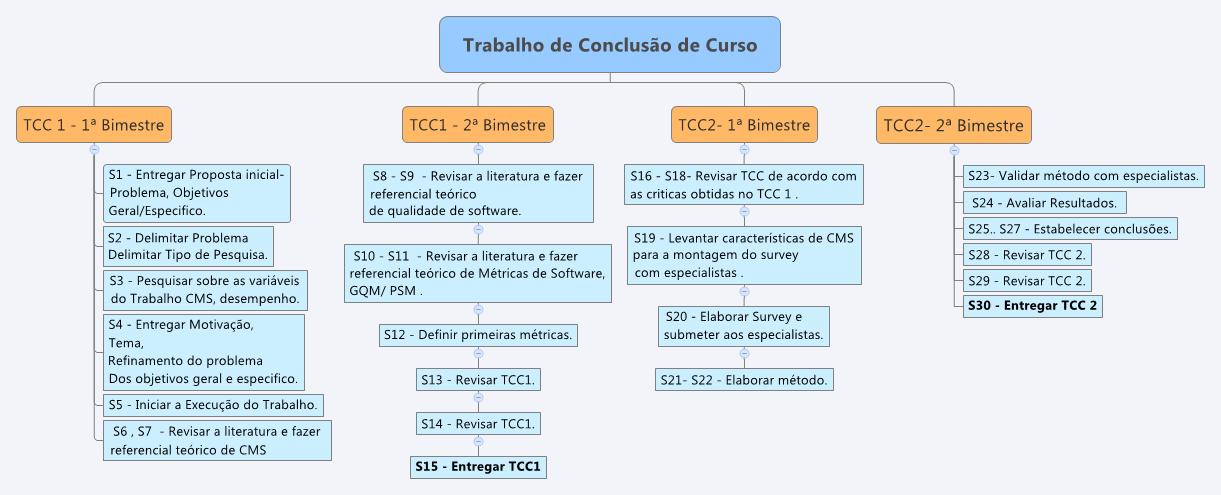
\includegraphics[keepaspectratio=true,scale= 0.58]{figuras/EAP.png}
\caption{Estrutura Analítica do Projeto de TCC.}
\label{EAP}
\end{figure}
\end{landscape}

\section{Organização da Pesquisa}

O desenvolvimento da pesquisa será organizado em capítulos que se seguem da seguinte forma.

\begin{itemize}


\item No Capítulo \ref{CMS} serão abordados conceitos chaves para o estudo de CMSs. Alguns destes conceitos são: vantagens e desvantagens no uso de CMSs para o desenvolvimento web e os critérios de seleção para a escolha dos CMSs que serão objetos de estudo desta pesquisa.
 
\item No Capítulo \ref{Qualidade_de_Software} serão abordados conceitos básicos de qualidade de software e conceitos referentes a série ISO/IEC 25000 de normas SQuaRE.  

\item No Capítulo \ref{metrics} serão apresentados conceitos sobre métricas de software e métodos obtidos da literatura que são especializados na definição de medições, para o objetivo de avaliar as características que serão utilizadas na escolha de CMSs. Foram estudados os métodos: GQM (\textit{Goal, Question, Metric}) e o PSM (\textit{Pratical Software Measurement}).

\item No Capítulo \ref{aplicação} será apresentado o passo a passo para a construção do método proposto, que compreende desde o levantamento de características de CMS na literatura, a estruturação do método, até a validação por surveys das características levantadas e das métricas mapeadas.

\item No Capítulo \ref{final}  serão apresentadas as conclusões obtidas com a realização do trabalho e sugestões de trabalhos futuros.  
%
%\item No capitulo \ref{aplicação} será feito um GQM com o objetivo de definir preliminarmente as medições necessárias para compor o conjunto de métricas para avaliar CMSs conforme suas características de desempenho.
%\item
%\item O capítulo \ref{final} conterá as conclusões do trabalho de TCC1, assim como as considerações finais e trabalhos futuros que serão realizados no âmbito do TCC2.
\end{itemize}
%\textcolor{red}{Escrever o que vai ter cada um dos capítulos}
